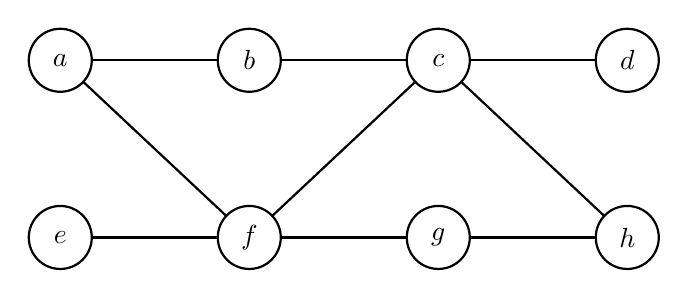
\begin{tikzpicture}[scale=1.5, >=stealth, every node/.style={circle, draw, thick, minimum size=8mm, inner sep=0pt}]
	% Top Row Vertices
	\coordinate (a) at (0, 1.5);
	\coordinate (b) at (1.6, 1.5);
	\coordinate (c) at (3.2, 1.5);
	\coordinate (d) at (4.8, 1.5);
	
	% Bottom Row Vertices
	\coordinate (e) at (0, 0);
	\coordinate (f) at (1.6, 0);
	\coordinate (g) at (3.2, 0);
	\coordinate (h) at (4.8, 0);
	
	% Edges
	\draw[thick] (0, 1.5) -- (1.6, 1.5); % a - b
	\draw[thick] (1.6, 1.5) -- (3.2, 1.5); % b - c
	\draw[thick] (3.2, 1.5) -- (4.8, 1.5); % c - d
	
	\draw[thick] (0, 0) -- (1.6, 0); % e - f
	\draw[thick] (1.6, 0) -- (3.2, 0); % f - g
	\draw[thick] (3.2, 0) -- (4.8, 0); % g - h
	
	\draw[thick] (0, 1.5) -- (1.6, 0); % a - f
	\draw[thick] (1.6, 0) -- (3.2, 1.5); % f - c
	\draw[thick] (3.2, 1.5) -- (4.8, 0); % c - h
	
	% Nodes drawn on top of lines
	\node[fill=white] at (a) {$a$};
	\node[fill=white] at (b) {$b$};
	\node[fill=white] at (c) {$c$};
	\node[fill=white] at (d) {$d$};
	
	\node[fill=white] at (e) {$e$};
	\node[fill=white] at (f) {$f$};
	\node[fill=white] at (g) {$g$};
	\node[fill=white] at (h) {$h$};
	\end{tikzpicture}